%\documentclass[iop]{emulateapj-rtx4}
% \shortauthors{French $\&$ Wakker}
%
%\usepackage{graphicx}
%\usepackage{subfigure}
%\usepackage{hyperref}
%\usepackage{amsmath}


%%%%%%%%%%
\documentclass[twocolumn,tighten]{aastex62}
%\documentclass{aastex6}
%\usepackage{emulateapj-rtx4}
%\usepackage{emulateapj}

 \shortauthors{French $\&$ Wakker}
\usepackage{graphicx}
\usepackage{subfigure}
\usepackage{amsmath}

%\usepackage{dblfloatfix}

%\usepackage{longtable}
%\usepackage{deluxetable}


\newcommand{\kms}{$\rm km\, s^{-1}$}
\newcommand{\HI}{\mbox{H\,{\sc i}} }

%\newcommand{\HI}{H\,{\sc i}}


\newcommand{\I}{\,{\sc i}}
\newcommand{\II}{\,{\sc ii}}
\newcommand{\III}{\,{\sc iii}}
\newcommand{\IV}{\,{\sc iv}}
\newcommand{\V}{\,{\sc v}}
\newcommand{\VI}{\,{\sc vi}}


\graphicspath{{figures//}}

\begin{document}

\title{The environmental dependence of low-$z$ Ly$\alpha$ absorption}

%Do Ly$\alpha$ absorbers co-rotate with galaxies?}

\author{David M. French, Bart P. Wakker}

\affil{Department of Astronomy, University of Wisconsin, Madison, WI 53706, USA}

\begin{abstract}
We present the results of a large-scale study of the Ly$\alpha$-probed CGM of nearby galaxies. We have identified \textbf{XXXX} Ly$\alpha$ absorbers in the redshift range $0 \leq z \leq 0.033$ and correlated their positions with the surrounding galaxy environment, leading to a sample of \textbf{XXXX} Ly$\alpha$ component-galaxy pairs, representing the largest-to-date dataset of it's kind. By employing the likelihood-based matching scheme of \cite{french2017}, we quantify the absorber-galaxy spacial correlation and identify 4 distinct absorber sub-samples. We find that absorber equivalent width and Doppler-b parameter are enhanced with increasing proximity to galaxies.

\end{abstract}


\keywords{galaxies:intergalactic medium, galaxies:evolution, galaxies:halos, quasars: absorption lines}


\section{INTRODUCTION}

The relationship between high column-density \HI absorption ($N(\HI) \gtrsim 10^{14} ~\rm cm^{-2}$) and galaxies has been well studied in the past several decades (e.g., \citealt{lanzetta1995, bowen1996, chen2003, chen2008, rubin2010, rubin2012, steidel2010, prochaska2011b}). \textbf{What do these studies find?} Relatively few studies have probed the $\rm Ly\alpha$-forest - galaxy relationship below this column density however (e.g., \citealt{wakker2009, french2017, bowen2002}). The most obvious reason for this is due to the technically demanding nature of detecting these weak absorption systems. The installation of the Cosmic Origins Spectrograph (COS) on the Hubble Space Telescope (\emph{HST}) in ??2011?? however has finally opened a window to study this rich reservoir of intergalactic gas.  Thanks to the high throughput and sensitivity available with COS, a large number of distant quasi-stellar objects (QSOs) have been observed with sufficiently high signal-to-noise for a large variety of science priorities. 

...


The second major challenge for galaxy-absorber correlation studies is obtaining data on the galaxies. While the resolution of absorption line spectroscopy is redshift-independent (e.g., a $N(\HI) \gtrsim 10^{13}  ~\rm cm^{-2}$ $\rm Ly\alpha$ absorber is just as readily detected at $z\sim0$ as at $z\sim 1$), detecting and classifying galaxies is a photometric exercise whose difficulty rapidly increases with redshift. Thus, while we wish to include all absorption systems in any particular sightline observation to maximize our sample size, we are instead limited by our ability to produce a matching galaxy sample. Different studies have gone about tackling this issue in different ways. ...


To make progress here we have completed the largest-to-date survey of low-$N$(\HI) $\rm Ly\alpha$ absorbers in the local Universe and their relationship to nearby galaxies. This survey is made possible by taking advantage of the large archival sample of COS QSO sightlines, and the high completeness of existing galaxy data in the redshift range $cz \leq 10,000$ \kms. In Section 2 we present the datasets, sample selection, and galaxy-absorber matching methods. In Section 3 we present and discuss the results of the galaxy-absorber correlation, and in Section 4 we offer our conclusions and discuss areas of future work.



\section{DATA ANALYSIS}
In this section we discuss the selection and reduction of our sample of archival QSO spectra taken by the Cosmic Origins Spectrograph (COS) on \textit{HST}. There currently exist over 700 COS spectra in the Barbara A. Mikulski Archive for Space Telescopes (MAST) with G130M exposures which cover the $\rm Ly\alpha$ transition in our survey's redshift range ($cz \leq 10,000$ \kms). In order to choose the most useful spectra for our purposes, we first sort them by signal-to-noise (SN) and make a cut at approximately SN=10. A signal-to-noise of approximately 10 or higher measured near $\rm 1238 \AA$ allows us to detect an absorption feature down to an equivalent width of $\rm \sim 50 m\AA$ at $5\sigma$. We then correlate the resulting (SN$\gtrsim 10$) sample with our galaxy catalog (see \ref{chapter1}), and sort the spectra by proximity to a galaxy. While this introduces a bias against void or isolated absorption features, we are presently most interested in the absorber-galaxy relation and therefore choose this method to maximize the associated absorber-galaxy sample size. Finally, from this galaxy-proximity sorted spectra list we choose 264 targets based on the relative ease of spectral feature identification. Data reduction, continuum fitting and line measurement are then conducted in an identical fashion to \cite{french2017}. Table \ref{QSOsample} summarizes the QSO targets included in this work.


\startlongtable
\begin{deluxetable*}{l l l l l l l}
\tabletypesize{\scriptsize}
%\setlength{\tabcolsep}{0.15in}
\tablecolumns{7}
%\tablewidth{2.0pt}
\tablecaption{Summary of QSO Sample\label{QSOsample}}
\tablehead{
\colhead{Target}  		&  \colhead{Galaxy} 			&  \colhead{R.A.}  		&  \colhead{Dec.}		& \colhead{z} 	&  \colhead{Program} &  \colhead{${T_{\rm exp}}$}	\\
			  		&          					&  			 		& 		  			& 		     	&				  & \colhead{(ks)}}
\colnumbers
\startdata
1H0419-577  				&      NGC1566  		&      04 26 00.7  		&	-57 12 02.0  		&   0.10400  	& 11686		& 20429	\\
2E1530+1511				&	NGC5951			&	15 33 14.3		&	+15 01 03.0		&   0.09000	& 14071		& 9348	\\
3C232					&	NGC3067			&	09 58 20.9		&	+32 24 02.0		&   0.5306	0	& 8596		& 44662	\\
3C273.0  					&	NGC4536  		&      12 29 06.7  		&	+02 03 09.0 		&   0.15834  	& 12038		& 4002	\\
CSO295					&	NGC3432			&	10 52 05.6		&	+36 40 40.0		&   0.60900	& 14772		& 1088	\\
CSO1208					&	NGC3726			&	11 40 47.9			&	+46 22 05.0		&   0.11500	& 14729		& 3052	\\
FBQSJ0908+3246			&	NGC2770			&	09 08 38.8		&	+32 46 20.0		&   0.25989	& 14240		& 7430	\\
H1101-232  				&      NGC3513  		&      11 03 37.7  		&	-23 29 31.0  		&   0.18600  	& 12025		& 13341	\\
HE0429-5343  				&      NGC1566  		&      04 30 40.0  		&	-53 36 56.0 		&   0.04001  	& 12275		& 2067	\\
%HE0435-5304  			&      NGC1566  		&      04 36 50.9  		&      -52 58 47.0  		&   0.42616  	& 11520		& 8372	\\
%HE0439-5254  			&      NGC1566  		&      04 40 12.0  		&	-52 48 18.0  		&   1.05300  	& 11520		& 8402	\\
HE1228+0131  				&      NGC4536  		&      12 30 50.0  		&	+01 15 23.0  		&   0.11700  	& 11686		& 11036	\\
MRC2251-178  			&      MCG-03-58-009  	& 	22 54 05.9  		&	-17 34 55.0  		&   0.06609  	& 12029		& 5515	\\
MRK335					&	NGC7817			&	00 06 19.5		&	+20 12 11.0		&   0.02578	& 11524		&  5122	\\
MRK771					&	NGC4529			&	12 32 03.6		&	+20 09 30.0		&   0.06301	& 12569		& 1868	\\
MRK876					&	NGC6140			&	16 13 57.2		&	+65 43 11.0		&   0.12900	& 11524		& 12579	\\
%MS1047.3+3518			&	NGC3432			&	10 50 10.9		&	+35 02 02.0		&   0.04125	& 8316		&  8301	\\
PG0804+761				&	UGC04238		&	08 10 58.7		&	+76 02 43.0		&   0.10200	& 11686		& 5510	\\
PG1259+593				&	UGC08146		&	13 01 12.9		&	+59 02 07.0		&   0.4778	0	& 11541		&  9200	\\
PG1302-102  				&      NGC4939  		&      13 05 33.0  		&	-10 33 19.0  		&   0.27840  	& 12038		& 5979	\\
QSO1500-4140  			&      NGC5786  		&      15 03 34.0  		&	-41 52 23.0  		&   0.33500  	& 11659		& 9258	\\
%RBS567  				&      NGC1566  		&      04 39 38.7  		&	-53 11 31.0  		&   0.24300  	& 11520		& 8176	\\
RBS1503					&	NGC5907			&	15 29 07.5		&	+56 16 07.0		&   0.09900	& 12276		&  1964	\\
RBS1768  				&      ESO343-G014  	&   	21 38 49.9  		&	-38 28 40.0  		&   0.18299  	& 12936		& 6962	\\
RBS2000  				&      IC5325  			&      23 24 44.7  		&	-40 40 49.0  		&   0.17359  	& 13448		& 5046	\\
%RX\_J1002.9+3240		&	NGC3067			&	10 02 54.5		&	+32 40 39.0		&   0.83000	& 12603		&  7713	\\
RX\_J1017.5+4702			&      NGC3198			&	10 17 31.0		&	+47 02 25.0  		&   0.33544  	& 13314		& 8655     \\
RX\_J1054.2+3511			&	NGC3432			&	10 54 16.2		&	+35 11 24.0		&   0.20300	& 14772		&  533	\\
%RX\_J1117.6+5301			&	UGC06446		&	11 17 40.5			&	+53 01 51.0		&   0.15871	& 14240		&  4943	\\
RX\_J1117.6+5301  			&      NGC3631  		&      11 17 40.5  		&   	+53 01 51.0  		&   0.15871  	& 14240  		&  4943    \\
RX\_J1121.2+0326  			&      CGCG039-137, NGC3633 		&   	11 21 14.0  		&	+03 25 47.0 		&   0.15200  	& 12248		& 2695	\\
%RX\_J1121.2+0326  		&      NGC3633  		&	11 21 14.0  		&	+03 25 47.0 		&   0.15200  	& 12248		& 2695	\\
RX\_J1142.7+4625			&	NGC3726			&	11 42 41.2			&	+46 24 36.0		&   0.11500	& 14772		&  2368	\\
RX\_J1236.0+2641			&	NGC4565			&	12 36 04.0		& 	+26 41 36.0		&   0.20920	& 12248		& 4235	\\
%SBS1116+523			&	UGC06399		&	11 19 47.9			&	+52 05 53.0		&   0.35568	& 14240		&  4949	\\
SBS1116+523				&	NGC3631			&	11 19 47.9			&	+52 05 53.0		&   0.35568	& 14240		&  4949	\\
SBS1503+570				&	NGC5907			&	15 04 55.6		&	+56 49 20.0		&   0.35894	& 12276		&  5163	\\
SDSSJ091052.80+333008.0	&	NGC2770			&	09 10 52.8		&	+33 30 08.0		&   0.11631	& 14240		&  7442	\\
SDSSJ091127.30+325337.0	&	NGC2770			&	09 11 27.3			&	+32 53 37.0		&   0.29038	& 14240		&  10028	\\
SDSSJ095914.80+320357.0	&	NGC3067			&	09 59 14.8		&	+32 03 57.0		&   0.56462	& 12603		&  2273	\\
%SDSSJ101622.60+470643.0	&	NGC3198			&	10 16 22.6		&	+47 06 43.0		&   0.82222	& 11598		& 4906  	\\
SDSSJ104335.90+115129.0	&	NGC3351			&	10 43 35.9		&	+11 05 29.0		&   0.79400	& 14071		& 4736	\\
%SDSSJ112005.00+041323.0  & 	NGC3633  		&      11 20 05.0  		&	+04 13 23.0 		&   0.54689  	& 12603		& 4708	\\
%SDSSJ112224.10+031802.0	&	NGC3633			&	11 22 24.1			&	+03 18 02.0		&   0.47528	& 12603		& 7588	\\
%SDSSJ112224.10+031802.0  & 	CGCG039-137 		&  	11 22 24.1  		&	+03 18 02.0 		&   0.47528  	& 12603		& 7588	\\
SDSSJ111443.70+525834.0  	& 	NGC3631  		&      11 14 43.7  		&   	+52 58 34.0  		&   0.07921  	& 14240  		& 13440   \\
SDSSJ112439.50+113117.0	&	NGC3666			&	11 24 39.4			&	+11 31 17.0		&   0.14300	& 14071		& 10427	\\
SDSSJ112448.30+531818.0	&	UGC06446, NGC3631		&	11 24 48.3			&	+53 18 19.0		&   0.53151	& 14240		& 7920	\\
%SDSSJ112632.90+120437.0	&	NGC3666			&	11 26 32.9			&	+12 04 37.0		&   0.97700	& 13314		& 8289	\\
%SDSSJ112756.70+115427.0	&	NGC3666			&	11 27 56.8			&	+11 54 27.0		&   0.50900	& 14145		& 5146	\\
SDSSJ135726.27+043541.4  	&	NGC5364  		&      13 57 26.3  		&	+04 35 41.0  		&   1.23453  	& 12264		& 14148	\\
SDSSJ151237.15+012846.0  	& 	UGC09760  		&      15 12 37.2  		&	+01 28 46.0  		&   0.26625  	& 12603		& 7590	\\
%SDSSJ152053.59+571122.1	&	NGC5907			&	15 20 53.7		&	+57 11 23.0		&   0.02952	& 13654		&  3753	\\
TON1009					&	NGC2770			&	09 09 06.2		&	+32 36 30.0		&   0.81028	& 12603		&  4740	\\
TON1015					&	NGC2770			&	09 10 37.0		&	+33 29 24.0		&   0.35400	& 14240		&  4774	\\
\enddata
%\tablenotetext{a}{Total exposure time and S/N ratio is given for multi-orbit exposures.}
\tablecomments{Summary of COS targets in this study. \textbf{THIS IS JUST A PLACEHOLDER}}
\end{deluxetable*}




In this sample of 264 QSOs we have detected 1135 Ly$\alpha$ absorbers. Figures \ref{allsky_2500} and \ref{allsky_7500} show all-sky maps of the positions of all absorbers split into 4 velocity bins ($v_{\rm Ly\alpha} = 0 - 2500$, $2501 - 5000$, $5001 - 7500$, and $7501 - 10,000$ \kms). The distribution of galaxies in the same velocity ranges are include here also (galaxies are plotted as small circles, absorbers as stars; see \textbf{Chapter 1}). Comparing by-eye the galaxy to absorber positions and velocities within each velocity range, we see that the Ly$\alpha$ absorbers broadly trace the locations of the galaxies. If the current Lambda Cold Dark Matter ($\Lambda$CDM) cosmology is to be believed, this should not be remarkably surprising. The baryons from which galaxies are built and those found within the IGM and traced by $\rm Ly\alpha$ absorption should both follow the underlying potential produced by the Dark Matter, and should therefore be found in similar places. Beyond this big-picture result however, we want to know how the absorbers react to the presence of the galaxies on a more local scale.


\begin{figure*}
\centering
  \subfigure[]{\includegraphics[width=0.99\linewidth]{2500kms_galaxies-True.pdf}}\label{allsky_2500}
  \subfigure[]{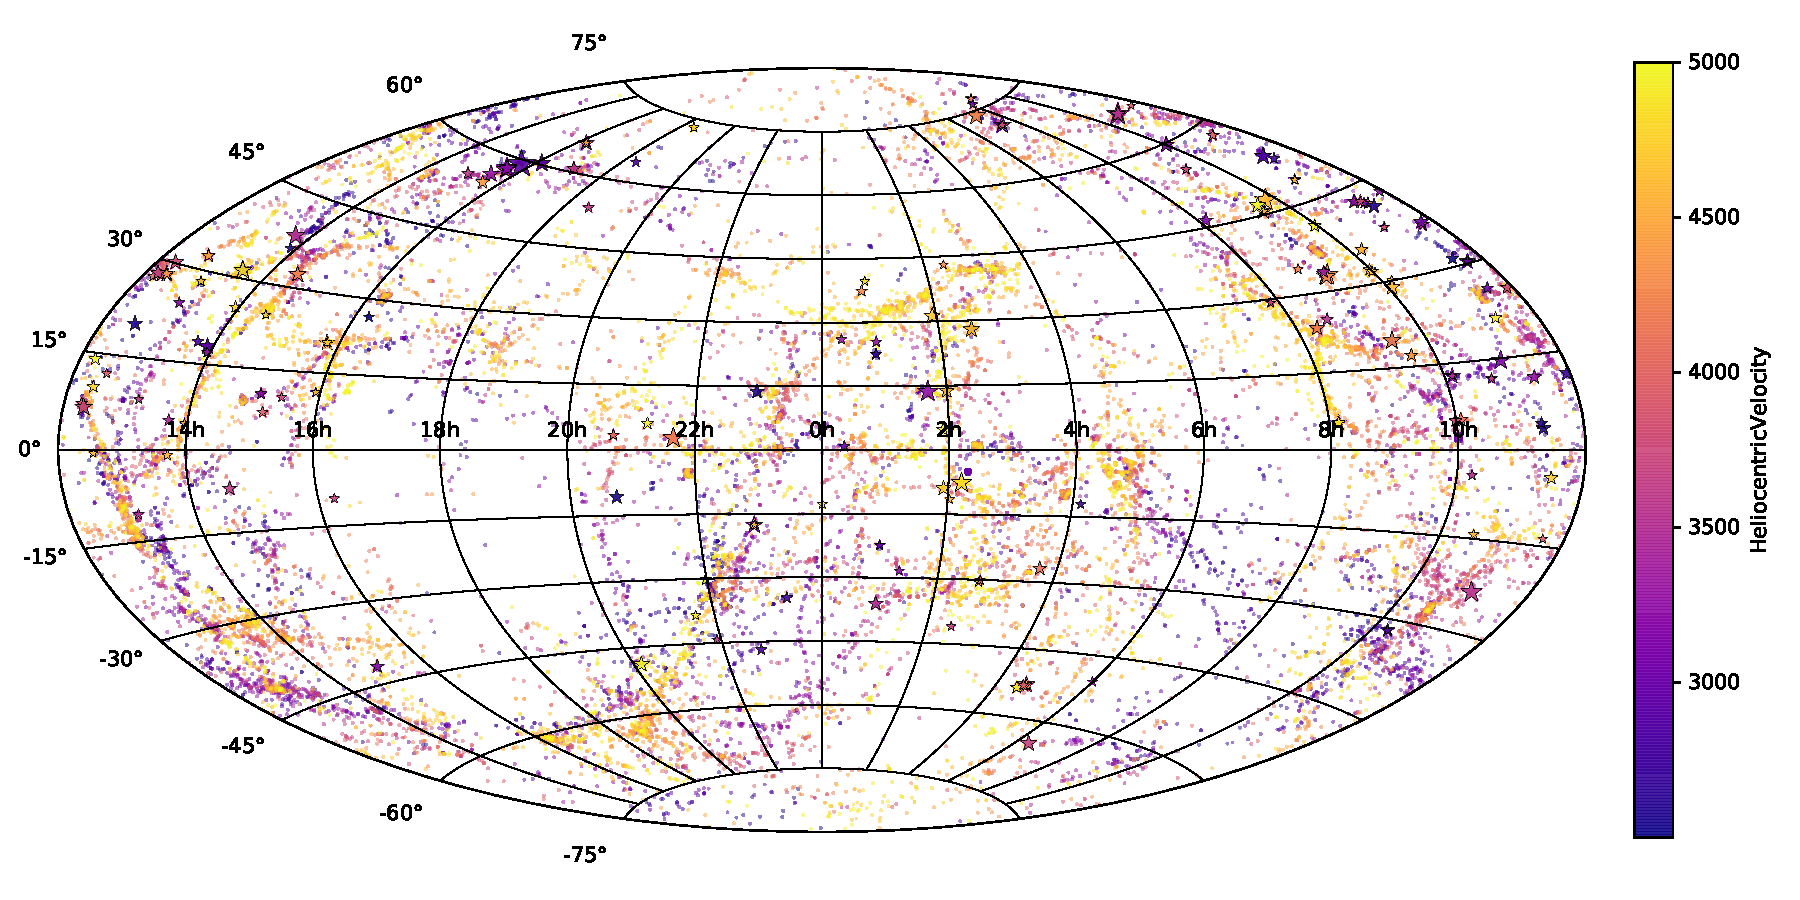
\includegraphics[width=0.99\linewidth]{5000kms_galaxies-True.pdf}}\label{allsky_5000}
  \caption{\small{All sky maps of the locations of all absorbers and galaxies. Absorbers are plotted as stars and scaled in size based on their EW. Galaxies are plotted as dots. The colors of both galaxies and absorbers are mapped to their heliocentric velocities. (a) All galaxies and absorbers in the velocity range $450 \leq cz \leq 2500$ \kms. (b) All galaxies and absorbers in the velocity range $2500 < cz \leq 5000$ \kms.}}
\vspace{0pt}
\end{figure*}


\begin{figure*}
\centering
  \subfigure[]{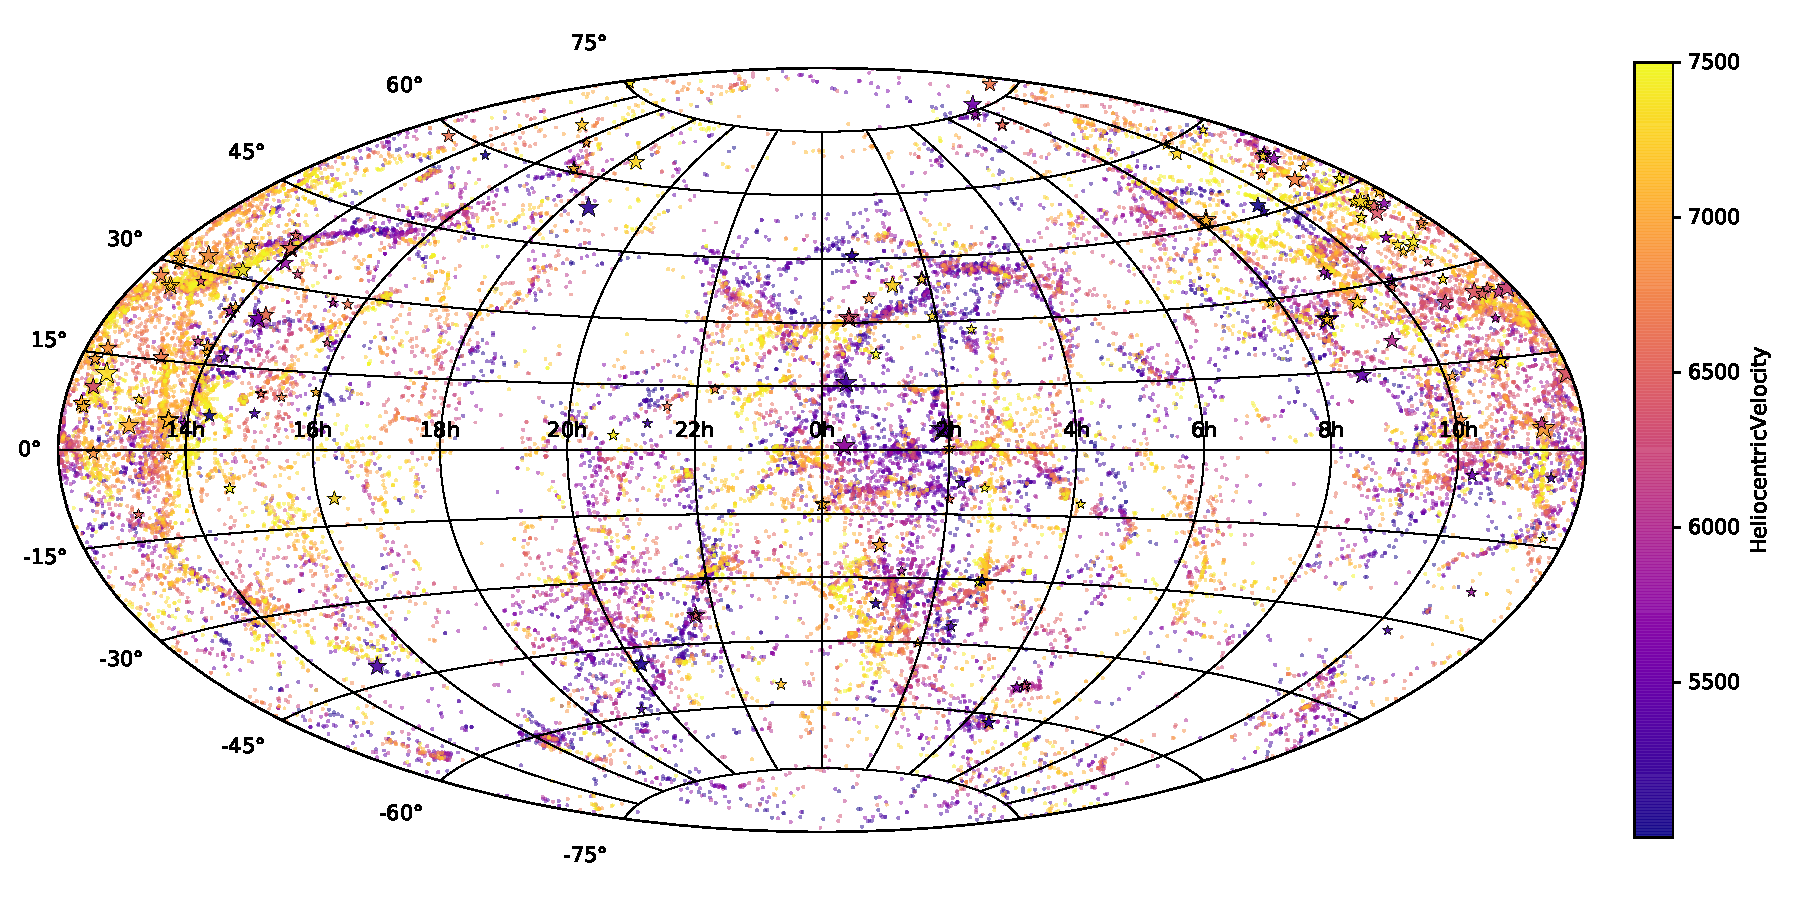
\includegraphics[width=0.99\linewidth]{7500kms_galaxies-True.pdf}}\label{allsky_7500}
  \subfigure[]{\includegraphics[width=0.99\linewidth]{10000kms_galaxies-True.pdf}}\label{allsky_10000}
  \caption{\small{All sky maps of the locations of all absorbers and galaxies. Absorbers are plotted as stars and scaled in size based on their EW. Galaxies are plotted as dots. The colors of both galaxies and absorbers are mapped to their heliocentric velocities. (a) All galaxies and absorbers in the velocity range $5000 < cz \leq 7500$ \kms. (b) All galaxies and absorbers in the velocity range $7500 < cz \leq 10,000$ \kms.}}
\vspace{0pt}
\end{figure*}




\subsection{Sub-sample selection}
As first introduced in \cite{french2017}, we employ a unique likelihood method for objectively matching absorbers with nearby galaxies in a consistent, analytical manner. We define likelihood, $\mathcal{L}$, as follows: 

\begin{equation}
\mathcal{L} = A \times e^{-(\frac{\rho}{R_{eff}})^2} \times e^{-(\frac{\Delta v}{v_{norm}})^2},
\label{likelihood}
\end{equation}

where $A$ is a normalization constant, $\rho$ is the impact parameter between a galaxy and sightline, $R_{\rm eff}$ is one of two possible ``effective - radii" we use for the galaxy (virial radius and $D^{1.5}$, or diameter to the 1.5 power), $\Delta v$ is the velocity separation between absorber and galaxy heliocentric, and $v_{norm}$ is a velocity normalization (equal to one of 150, 200, or 250). We calculate $\mathcal{L}$ for every absorber-galaxy combination, which then gives us a single number as a three-dimensional proxy for the physical separation between the two. We furthermore explore the results of adjusting the several possible $\mathcal{L}$ normalizations. We calculate $\mathcal{L}$ with $R_{eff}$ equal to $R_{vir}$ and $D^{1.5}$ and $v_{norm}$ equal to 150, 200, and 250. For each of these combinations, we also calculate a variant with $A =1$ and another with $A = 2$ if $R_{eff} \ge \rho$, and $A=1$ otherwise. Table \textbf{TABLE} summarizes the resulting subsets for each of these combinations.



%($A=1$, $R_{eff} = R_{vir}$, $v_{norm} = 200$, $\mathcal{L}_{min} = 0.01$)

% this table is from pickle version 8 results
\begin{deluxetable*}{| l | c | c | c | c | c |}
\setlength{\tabcolsep}{0.1in}
\tablecolumns{8}
\tabletypesize{\scriptsize}
%\tablewidth{1pt}
\tablecaption{Summary of $\mathcal{L}$ Variants \label{likelihood_variants}}
\tablehead{
\colhead{$\mathcal{L}$ variant}  										&  \colhead{Isolated}		&  \colhead{$\mathcal{L}$-isolated}	&  \colhead{$\mathcal{L}$ - Assoc. (Isolated)}	&  \colhead{$\mathcal{L}$ - Assoc.}	&  \colhead{$\mathcal{L}$-Two+} 	}
\startdata
Standard															&	571				&	267						&	56								&	146						&	58						\\
\hline
$\mathcal{L}_{min} = 0.001$											&	571				&	227						&	69								&	167						&	65						\\
\hline
$D^{1.5}$, $\mathcal{L}_{min} = 0.001$ 									&	571				&	317						&	39								&	174						&	32						\\
\hline
$A=2~if~\rho \leq R_{vir}$, $\mathcal{L}_{min} = 0.001$						&	571				&	227						&	69								&	181						&	62						\\
\hline
$\mathcal{L}_{min} = 0.005$, $v_{norm} = 150$							&	571				&	265						&	58								&	148						&	63						\\
\hline
$\mathcal{L}_{min} = 0.005$, $v_{norm} = 250$							&	571				&	246						&	64								&	151						&	64						\\
\hline
\enddata
\tablecomments{A summary of the subset sizes resulting from varying the likelihood metric's normalization parameters.}
\vspace{-5pt}
\end{deluxetable*}


\section{Results \& Discussion}

First we explore the $\rm Ly\alpha$ detection fraction as a function of galaxy proximity. To calculate this, we start by correlating the position of every QSO with our galaxy sample. For every galaxy found within 1000 kpc in physical impact parameter of each sightline we then check if a $\rm Ly\alpha$ line appears in that sightline and within 400 \kms~of the galaxy's systemic velocity. This results in a detection fraction as a function of impact parameter. Additionally, we calculate the detection fraction as a function of likelihood, $\mathcal{L}$, in a similar manner. However, as we are calculating detection fraction without any a priori knowledge of the velocity of the absorption lines, the likelihood we calculate is simply $e^{-(\rho/R_{vir})^2}$, or only the impact parameter - virial radius portion of our usual likelihood function given by Eq. \ref{likelihood}. Note that this adjusted likelihood function is identical to Eq. \ref{1} if $\Delta v = 0$. We have plotted both detection fractions in Figure \ref{detection_fraction}. 




\subsection{Equivalent Width}

Here we explore the effect of environment on the equivalent width of our $\rm Ly\alpha$ absorber sample. 

\begin{figure*}[ht!]
        \centering
        \vspace{0pt}
        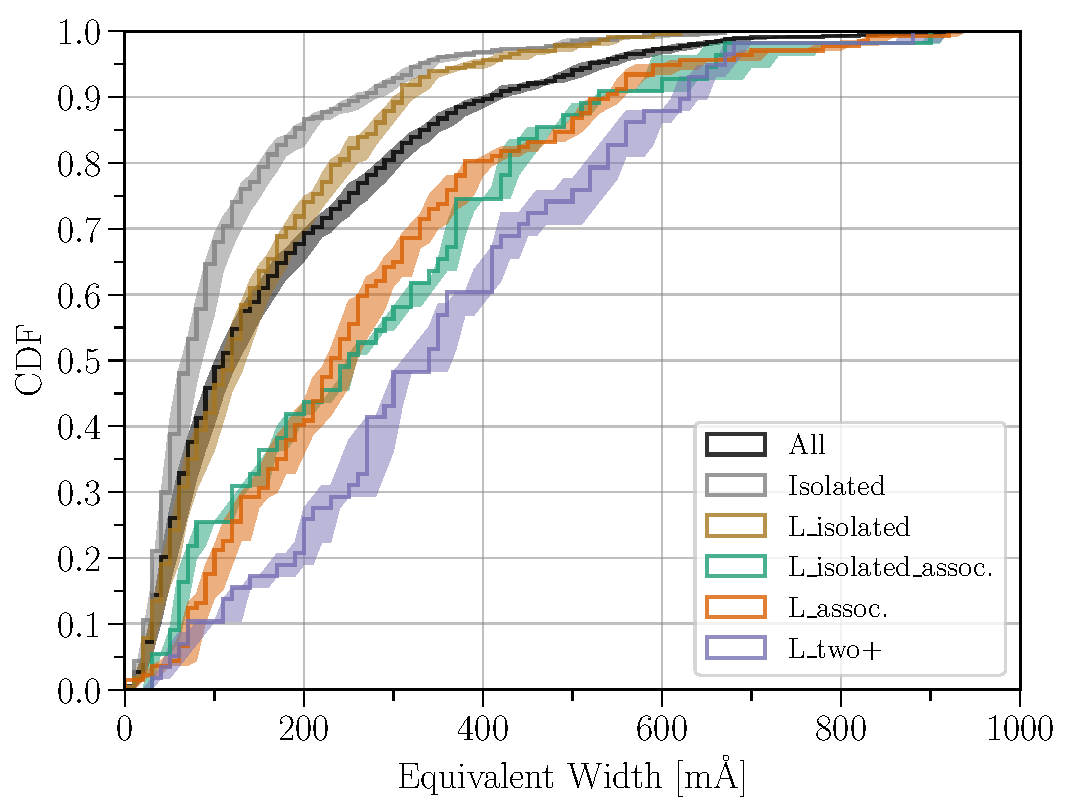
\includegraphics[width=0.95\textwidth]{hist(EW)_all6_bins10_6alt_min_maxEW_0_10000_err.pdf}
        \caption{\small{The equivalent width (EW) cumulative distribution function for each subset of our Ly$\alpha$ absorber sample. From the top-left corner to the bottom-right the curves are the fully isolated absorbers (grey), the absorbers isolated enough from any galaxy to not be likelihood-matched (brown), the full distribution (black), the absorbers likelihood-matched to a single, non-isolated galaxy (orange), the absorbers matched to a single, isolated galaxy (green), and the absorbers likelihood-matched with two or more galaxies (purple). The shaded region around each curve gives the EW measurement errors.}}
        \vspace{-5pt}
        \label{cdf_ew}
\end{figure*}


\subsection{Doppler b-parameter}

Here we explore the effect of environment on the Doppler b-parameter of our $\rm Ly\alpha$ absorber sample.
\begin{figure*}[ht!]
        \centering
        \vspace{0pt}
        \includegraphics[width=0.95\textwidth]{hist(b)_all6_bins1_6_min_maxEW_0_10000.pdf}
        \caption{\small{The Doppler b-parameter ($b$) cumulative distribution function for each subset of our Ly$\alpha$ absorber sample. From the top-left corner to the bottom-right the curves are the fully isolated absorbers (grey), the absorbers isolated enough from any galaxy to not be likelihood-matched (brown), the full distribution (black), the absorbers likelihood-matched to a single, non-isolated galaxy (orange), the absorbers matched to a single, isolated galaxy (green), and the absorbers likelihood-matched with two or more galaxies (purple). The shaded region around each curve gives the EW measurement errors.}}
        \vspace{-5pt}
        \label{cdf_b}
\end{figure*}




\subsection{Azimuth}

\subsection{Inclination}

Here we investigate the inclination dependence of $\rm Ly\alpha$ absorber properties.

As expected if this is the case, we also see an inclination dependence in the overall $\rm Ly\alpha$ detection fraction. For example, if absorbers are distributed in a perfectly spherical manner around galaxies, then we would expect just as many non-detections as detections at any given galaxy inclination and impact parameter from a sightline. We do not find this. Figure \ref{detection_fraction_inclination} shows the median inclinations for galaxies near positive or negative $\rm Ly\alpha$ detections as a function of both impact parameter and $\mathcal{L}$. In both cases, positive detections are predominantly found near more highly inclined galaxies than non-detections.



\begin{figure*}
\centering
  \subfigure[]{\includegraphics[width=0.49\linewidth]{detection_fraction_impact_inc_median_Lstarcut01-2.pdf}\label{detection_fraction_impact_inc}}
  \subfigure[]{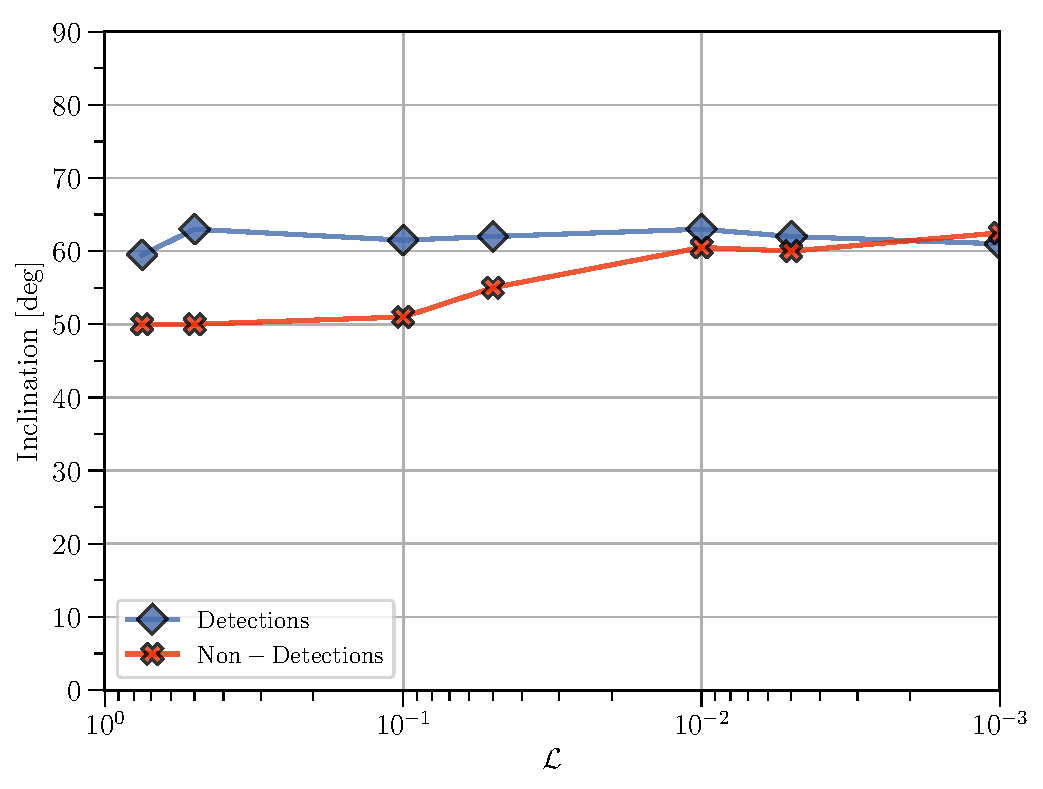
\includegraphics[width=0.49\linewidth]{detection_fraction_likelihood_inc_median_Lstarcut01-2.pdf}\label{detection_fraction_likelihood_inc}}
  \caption{\small{(a) The median inclination is shown for galaxies at a given impact parameter from a positive (blue-diamonds) or negative (red-crosses) $\rm Ly\alpha$ detection. (b) The median inclination is shown for galaxies at a given $\mathcal{L}$ from a positive (blue-diamonds) or negative (red-crosses) $\rm Ly\alpha$ detection.}}
  \label{detection_fraction_inclination}
\vspace{0pt}
\end{figure*}




\section{Future Work}

Cross-correlation functions \cite{chen2005}

Metals





\section{SUMMARY}
1. $\rm Ly\alpha$ absorbers with $\rm EW \lesssim 100 m\AA$ are ubiquitous, making up nearly $50\%$ of all $\rm Ly\alpha$ systems in the nearby Universe, and do not correlate strongly with environment ($70\%$ of these weak absorbers are isolated). 

% \begin{deluxetable*}{l l l l l l l l l l l}
%%\setlength{\tabcolsep}{0.05in}
%\tablecolumns{11}
%\tabletypesize{\scriptsize}
%%\tablewidth{0pt}
%\tablecaption{SALT Galaxy Observations\label{tab:params}}
%\tablehead{
%\colhead{Galaxy}	&  \colhead{R.A.}	&  \colhead{Dec.}  	&  \colhead{Measured $v_{\rm sys}$}& \colhead{Published $v_{\rm sys}$} & \colhead{Type} &  \colhead{Grating}	&  \colhead{$v_{\rm rot}$}	& \colhead{$v_{\rm rot} / \sin(\emph{i})$}	& \colhead{Obs. Date} & \colhead{$T_{\rm exp}$}  \\
%			  	&          			&  			 	& \colhead{(\kms)}  				& \colhead{(\kms)}  		     	   &				& 				&  \colhead{(\kms)}  		& \colhead{(\kms)}					&					& \colhead{(ks)} }
%\colnumbers
%\startdata
% CGCG039-137 	& 11 21 27.0		& +03 26 41.7		& $6918 \pm24$\				&	$6902 \pm 52^{a}$	& Scd		& PG2300			& $132 \pm 16$	& $139 \pm 26$			& 05 11 2016		& 700	\\ %done
% \hline
%\enddata
%\tablecomments{SALT targeted galaxies. Columns are as follows: 1) the galaxy name, 2), 3) R.A., Dec. in J2000, 4) galaxy systemic velocity, 5) morphological type (RC3), 6) RSS grating used, 7) approaching side velocity, 8) receding side velocity, 9) observation date, and 10) exposure time}
%\tablerefs{a. \cite{sdssDR3}; b. \cite{6dFDR3}; c. \cite{RC3}; d. \cite{mathewson1996}; e. \cite{koribalski2004}; f. \cite{lu1993}; g. \cite{grogin1998}; h. \cite{dinella1996}; i, \cite{giovanelli1997}}
% \label{salt_targets}
%\end{deluxetable*}



%%\begin{eqnarray}
%%	\nonumber
%%	\sigma^2 = \left( \frac{\partial v_{rot}}{\partial \lambda_{obs}} \right)^2 (\Delta \lambda_{obs})^2 + \\
%%	\nonumber
%%	\left(\frac{\partial v_{rot}}{\partial v_{sys}} \right)^2 (\Delta v_{sys})^2 + \\
%%	\left( \frac{\partial v_{rot}}{\partial i} \right)^2 (\Delta i)^2,
%%\end{eqnarray}



\acknowledgements

D. M. F. thanks \textbf{A BUNCH OF PEOPLE}.This research has made use of the NASA/IPAC Extragalactic Database (NED) which is operated by the Jet Propulsion Laboratory, California Institute of Technology, under contract with the National Aeronautics and Space Administration. Based on observations with the NASA/ESA \textit{Hubble Space Telescope}, obtained at the Space Telescope Science Institute (STScI), which is operated by the Association of Universities for Research in Astronomy, Inc., under NASA contract NAS 5-26555. \textbf{SALT ACKNOWLEDGEMENT}. Spectra were retrieved from the Barbara A. Mikulski Archive for Space Telescopes (MAST) at STScI. Over the course of this study, D.M.F. and B.P.W. were supported by grant XXXX

%AST-1108913, awarded by the US National Science Foundation, and by NASA grants \textit{HST}-AR-12842.01-A, \textit{HST}-AR-13893.01-A, and \textit{HST}-GO-14240 (STScI). 

\facility{HST (COS), SALT (RSS)}
\clearpage

%\nocite{*}
%\bibliography{rotation_bib}
%\bibliography{/Users/frenchd/Research/bib}{}
\bibliography{/Users/frenchd/Research/inclination/git_inclination/bib}{}
\bibliographystyle{apj}

\clearpage

\appendix

\end{document}
